\section{Casi d'uso}
I casi d'uso sono catalogati come:
\begin{center}
	UC[numero][caso]
\end{center}
dove:
\begin{itemize}
	\item \textit{UC} specifica che si sta parlando di un caso d'uso;
	\item \textit{numero} è assoluto e rappresenta un riferimento univoco al caso d'uso in questione;
	\item \textit{caso} individua eventuali diramazioni all'interno dello stesso caso d'uso.
\end{itemize}

\subsection{Framework}

\UC{Istanziazione della bubble generica}{UC1.35}

\begin{figure}[H]
	\centering
	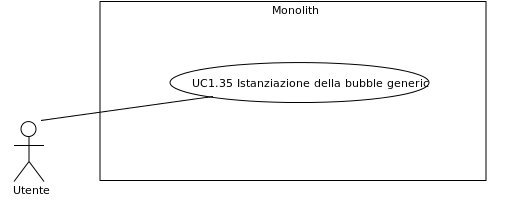
\includegraphics[width=15cm]{../../documenti/AnalisiDeiRequisiti/Diagrammi_img/uc1_35.png}
	\caption{\UCCaption{} Istanziazione della bubble generica}
\end{figure}

\begin{itemize}
	\item \textbf{Attori:}
	\\Utilizzatore del framework.
	\item \textbf{Scopo e descrizione:} 
	\\L'utilizzatore del framework può istanziare il contenitore \glossario{bubble generica}, il quale funge da contenitore dei vari elementi di input, output e di logica specificati all'interno del framework.
	\item \textbf{Flusso principale degli eventi:}
	\\L'utilizzatore del framework chiama il metodo per istanziare la bubble generica e la memoria ad essa associata.
	\item \textbf{Post-condizione:}
	\\È presente la bubble generica, compresa la sua memoria.
\end{itemize}

\UC{Interazione con database MongoDB}{UC2}

\begin{figure}[H]
	\centering
	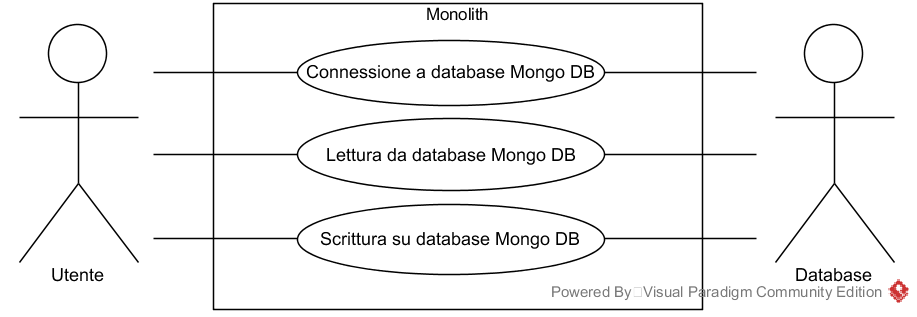
\includegraphics[width=15cm]{../../documenti/AnalisiDeiRequisiti/Diagrammi_img/Database.png}
	\caption{\UCCaption{} Interazione con database MongoDB}
\end{figure}

\begin{itemize}
	\item \textbf{Attori:}
	\\Utilizzatore del framework.
	\item \textbf{Scopo e descrizione:} 
	\\L'utilizzatore del framework interagisce con un database \glossario{MongoDB} esterno.
	\item \textbf{Precondizioni:}
	\begin{itemize}
		\item Avere già istanziato una bubble generica;
		\item Avere l'indirizzo di un database MongoDB con cui si desidera interagire.
	\end{itemize}
	\item \textbf{Flusso principale degli eventi:}
	\begin{itemize}
		\item L'utilizzatore del framework si connette al database MongoDB \ref{UC1.00};
		\item L'utilizzatore del framework effettua una lettura delle informazioni contenute all'interno del database MongoDB \ref{UC1.01};
		\item L'utilizzatore del framework effettua una scrittura sul database MongoDB \ref{UC1.02}.
	\end{itemize}
	\item \textbf{Post-condizione:}
	\\L'utilizzatore del metodo ha interagito con il database.
\end{itemize}

\begin{samepage}
\UCC[2]{Connessione a database MongoDB}{UC1.00}
\nopagebreak
\begin{figure}[H]
	\centering
	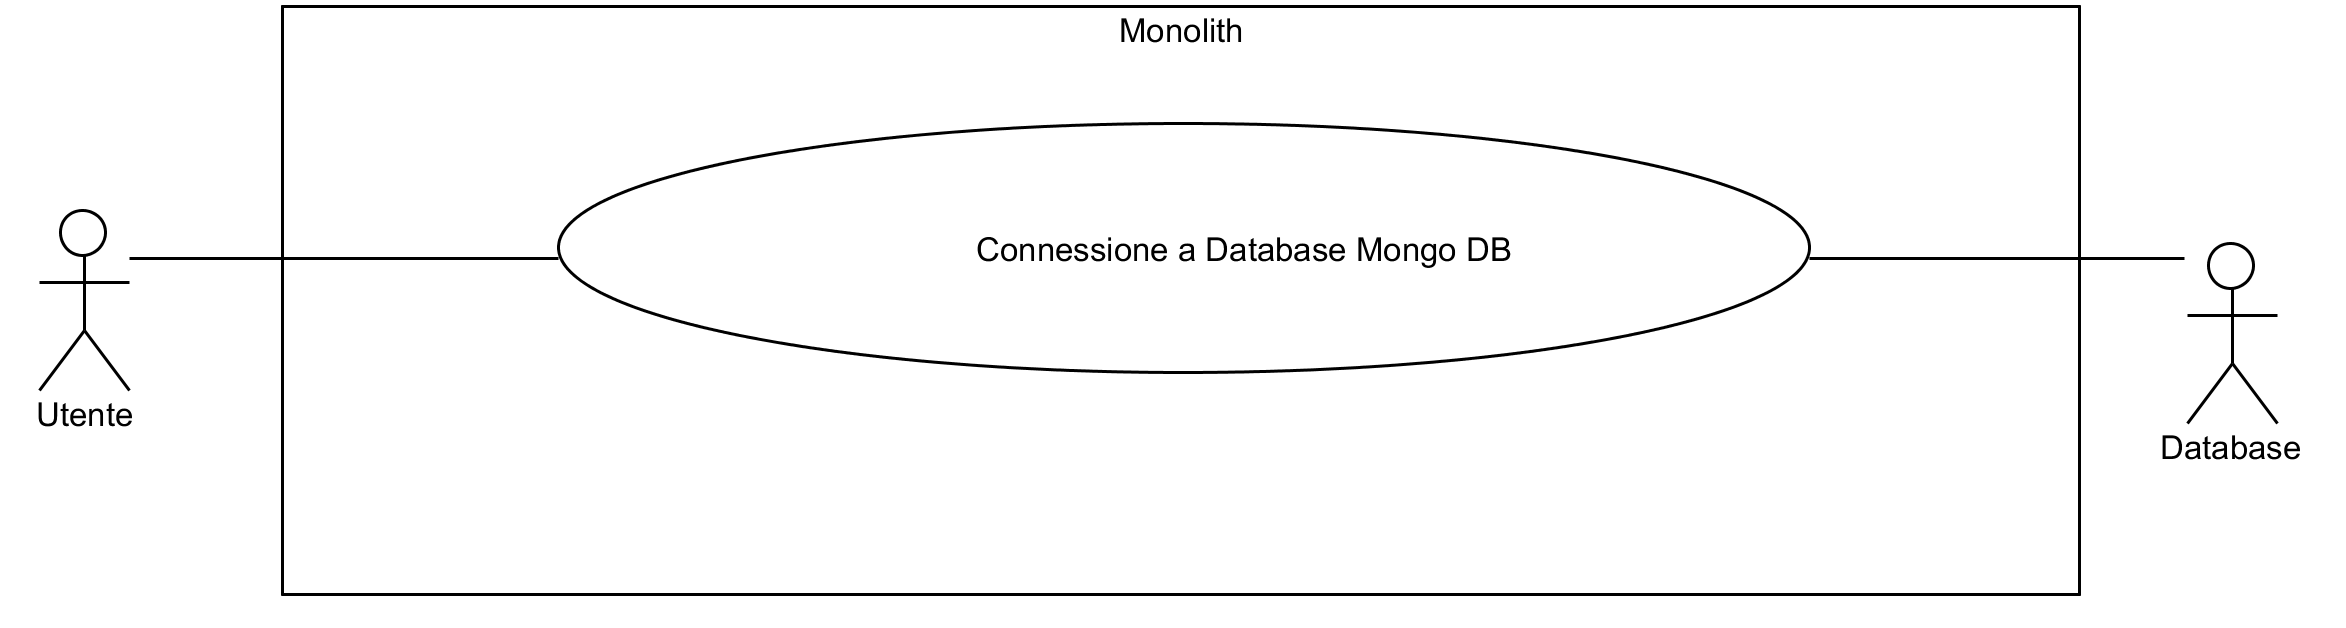
\includegraphics[width=15cm]{../../documenti/AnalisiDeiRequisiti/Diagrammi_img/uc1_00.png}
	\caption{\UCFCaption{} Connessione a database MongoDB}
\end{figure}
\end{samepage}

\begin{itemize}
\item \textbf{Attori:}
\\Utilizzatore del framework.
\item \textbf{Scopo e descrizione:} 
\\Connettersi ad un database MongoDB esterno all'applicazione.
\item \textbf{Precondizioni:}
	\begin{itemize}
		\item Avere già istanziato una bubble generica;
		\item Avere l'indirizzo del database MongoDB a cui si desidera connettersi.
	\end{itemize}
\item \textbf{Flusso principale degli eventi:}
\\L'utilizzatore passa l'indirizzo del database a cui connettersi al metodo che genera una connessione con il database MongoDB.
\item \textbf{Scenari alternativi:}
\\Non è possibile stabilire la connessione.
\item \textbf{Post-condizione:}
\\La bubble generica da cui è invocato il metodo è connessa al database.
\end{itemize}

\UCC[2]{Connessione a database MongoDB non possibile}{UC1.00.2}
\begin{itemize}
	\item \textbf{Attori:}
	\\Utilizzatore del framework.
	\item \textbf{Scopo e descrizione:} 
	\\Connettersi ad un database MongoDB esterno all'applicazione.
	\item \textbf{Precondizioni:}
	\begin{itemize}
		\item Avere già istanziato una bubble generica;
		\item Avere l'indirizzo del database MongoDB a cui si desidera connettersi.
	\end{itemize}
	\item \textbf{Flusso principale degli eventi:}
	\\L'utilizzatore passa l'indirizzo del database a cui connettersi al metodo che fallisce nel tentativo di stabilire una connessione con il database MongoDB.
	\item \textbf{Scenari alternativi:}
	\\La connessione avviene correttamente \ref{UC1.00}.
	\item \textbf{Post-condizione:}
	\\La bubble generica lancia un messaggio di errore e avvisa l'utente che la connessione non è riuscita.
\end{itemize}

\begin{samepage}
\UCF{Lettura da database MongoDB}{UC1.01}
\nopagebreak	
\begin{figure}[H]
	\centering
	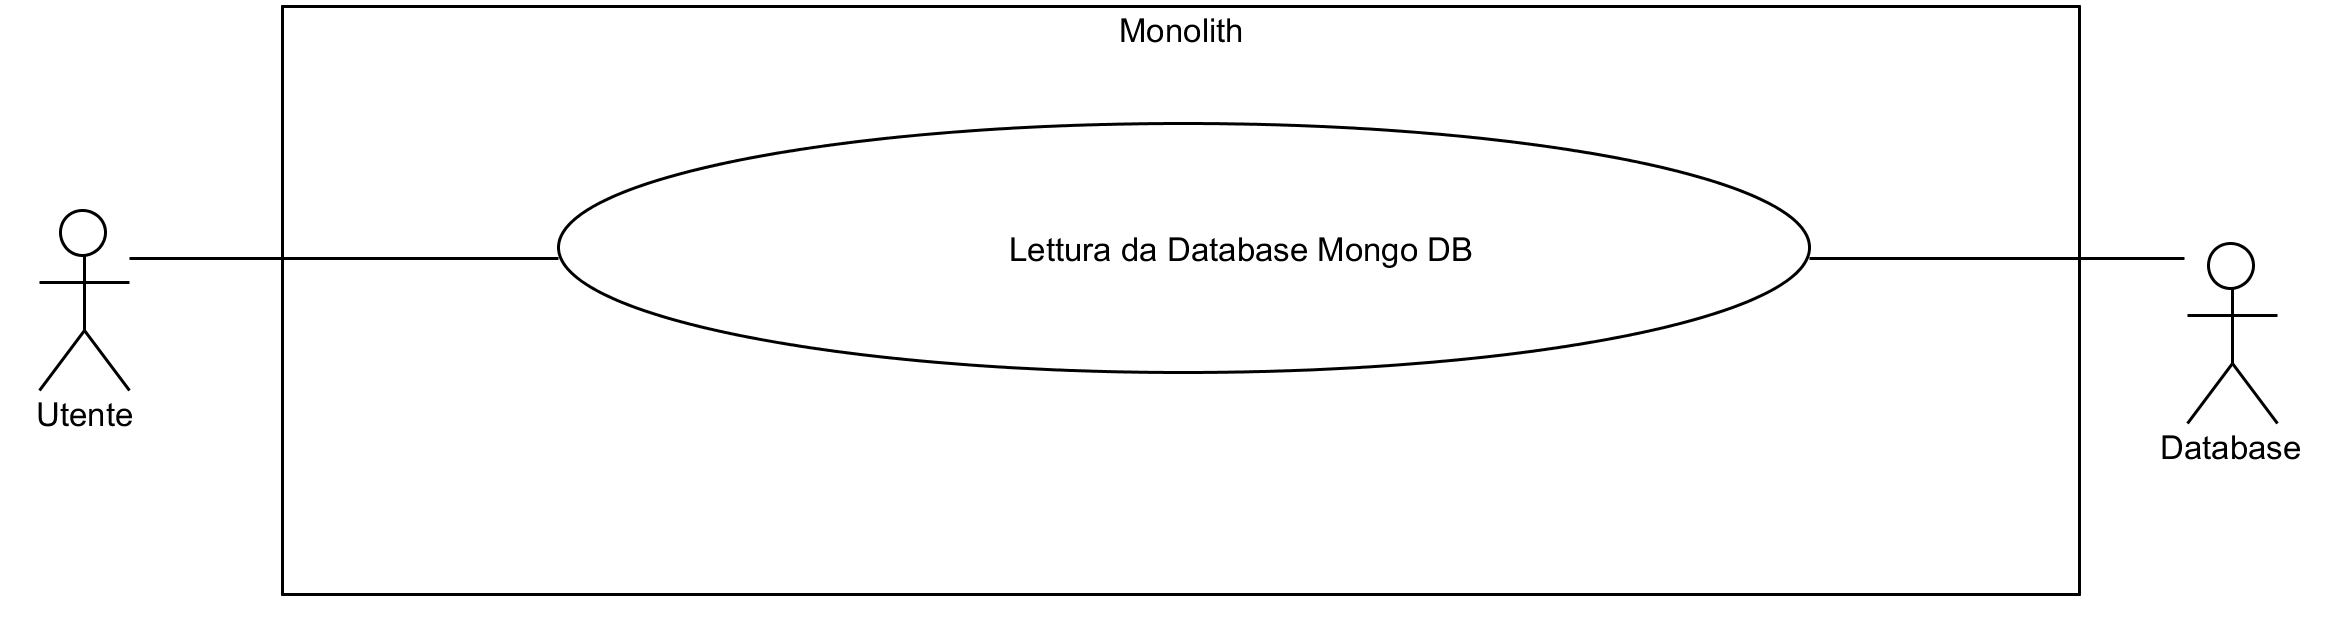
\includegraphics[width=15cm]{../../documenti/AnalisiDeiRequisiti/Diagrammi_img/uc1_01.png}
	\caption{\UCFCaption{} Lettura da database MongoDB}
\end{figure}
\end{samepage}

\begin{itemize}
	\item \textbf{Attori:}
	\\Utilizzatore del framework.
	\item \textbf{Scopo e descrizione:} 
	\\Prelevare dati dal database connesso alla bubble.
	\item \textbf{Precondizioni:}
	\begin{itemize}
		\item Avere già istanziato una bubble generica;
		\item La bubble è connessa al database MongoDB \ref{UC1.00};
		\item L'utilizzatore deve conoscere il nome della \glossario{collection} da cui prelevare i dati.
	\end{itemize}
	\item \textbf{Flusso principale degli eventi:}
	\\L'utilizzatore chiama il metodo su una bubble, il quale gli ritorna un oggetto \glossario{JSON} letto dal database, eventualmente assegnabile ad un campo della \glossario{bubble memory}.
	\item \textbf{Post-condizione:}
	\\I dati sono prelevati dal database e sono pronti all'uso nella bubble.
\end{itemize}

\begin{samepage}
\UCF{Scrittura su database MongoDB}{UC1.02}
\nopagebreak
\begin{figure}[H]
	\centering
	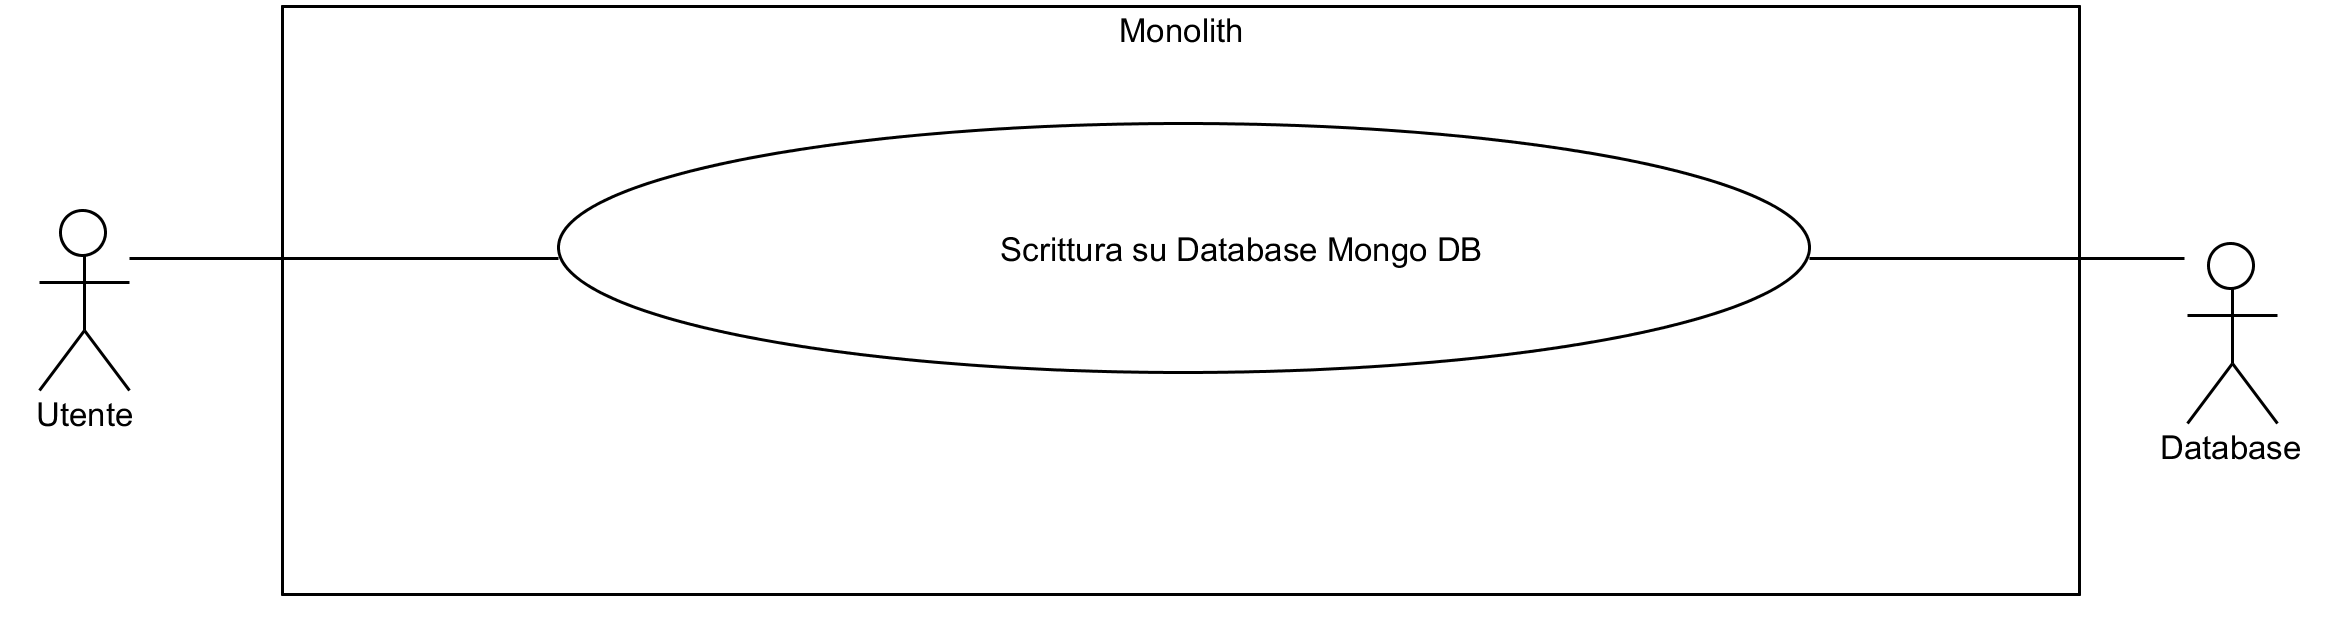
\includegraphics[width=15cm]{../../documenti/AnalisiDeiRequisiti/Diagrammi_img/uc1_02.png}
	\caption{\UCFCaption{} Scrittura su database MongoDB}
\end{figure}
\end{samepage}

\begin{itemize}
\item \textbf{Attori:}
\\Utilizzatore del framework.
\item \textbf{Scopo e descrizione:} 
\\Scrittura dati nel database connesso alla bubble.
\item \textbf{Precondizioni:}
\begin{itemize}
	\item Avere già istanziato una bubble generica;
	\item La bubble è connessa al database MongoDB \ref{UC1.00};
	\item L'utilizzatore deve conoscere il nome della collection da cui prelevare i dati.
\end{itemize}
\item \textbf{Flusso principale degli eventi:}
\\L'utilizzatore chiama il metodo su una bubble passandogli un oggetto \glossario{JavaScript}, serializzabile in JSON, e il metodo lo salva nel database.
\item \textbf{Post-condizione:}
\\I dati sono scritti nel database collegato.
\end{itemize}

\UC{Effettuare operazioni sugli elementi}{UC3}

\begin{figure}[H]
	\centering
	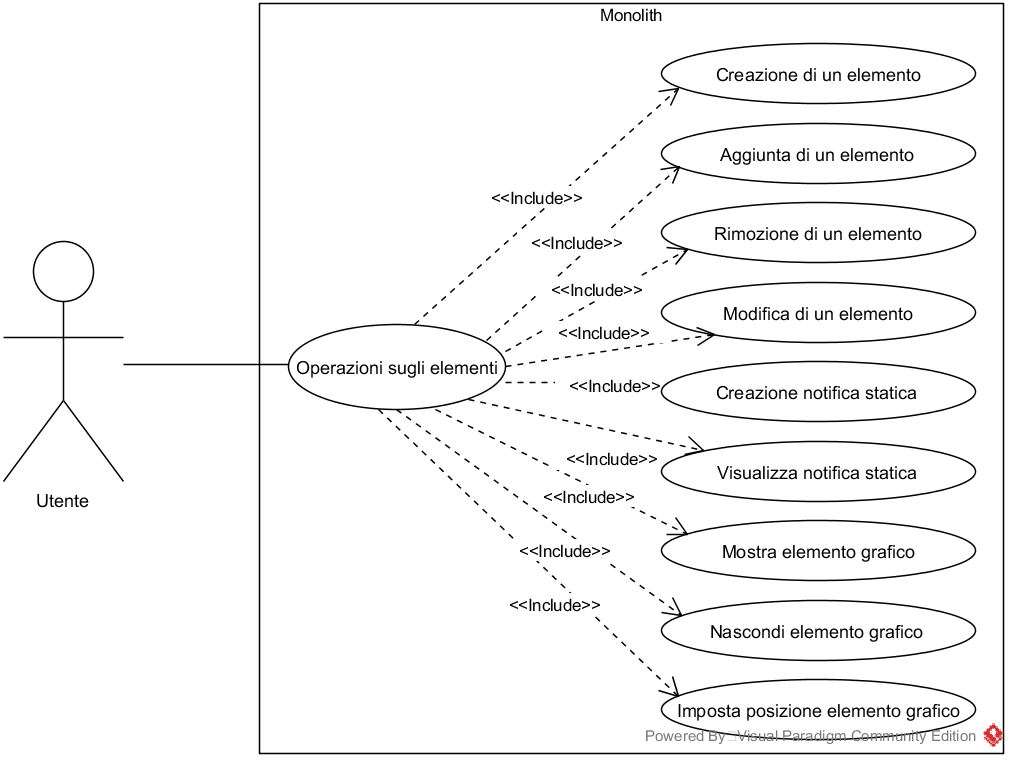
\includegraphics[width=15cm]{../../documenti/AnalisiDeiRequisiti/Diagrammi_img/operazioni.png}
	\caption{\UCCaption{} Effettuare operazioni sugli elementi}
\end{figure}

\begin{itemize}
	\item \textbf{Attori:}
	\\Utilizzatore del framework.
	\item \textbf{Scopo e descrizione:} 
	\\Effettuare una o più operazioni sugli elementi della bubble.
	\item \textbf{Precondizioni:}
	\begin{itemize}
		\item Avere già istanziato una bubble generica.
	\end{itemize}
	\item \textbf{Flusso principale degli eventi:}
	\begin{itemize}
		\item L'utilizzatore del framework crea un elemento \ref{UC3.01};
		\item L'utilizzatore del framework aggiunge un elemento alla bubble \ref{UC1.04};
		\item L'utilizzatore del framework rimuove un elemento dalla bubble \ref{UC1.03.1};
		\item L'utilizzatore del framework modifica un elemento della bubble \ref{UC1.05.1};
		\item L'utilizzatore del framework crea una notifica statica \ref{UC1.17};
		\item L'utilizzatore del framework rende visualizzabile da un utente una notifica statica \ref{UC1.18};
		\item L'utilizzatore del framework mostra un elemento grafico \ref{UC1.21};
		\item L'utilizzatore del framework nasconde un elemento grafico \ref{UC1.22};
		\item L'utilizzatore del framework imposta la posizione di un elemento grafico \ref{UC1.23}.
	\end{itemize}
	\item \textbf{Post-condizione:}
	\\Sono state apportate delle modifiche agli elementi della bubble.
\end{itemize}

\begin{samepage}
\UCF{Creazione di un elemento}{UC3.01}
\nopagebreak
\begin{figure}[H]
	\centering
	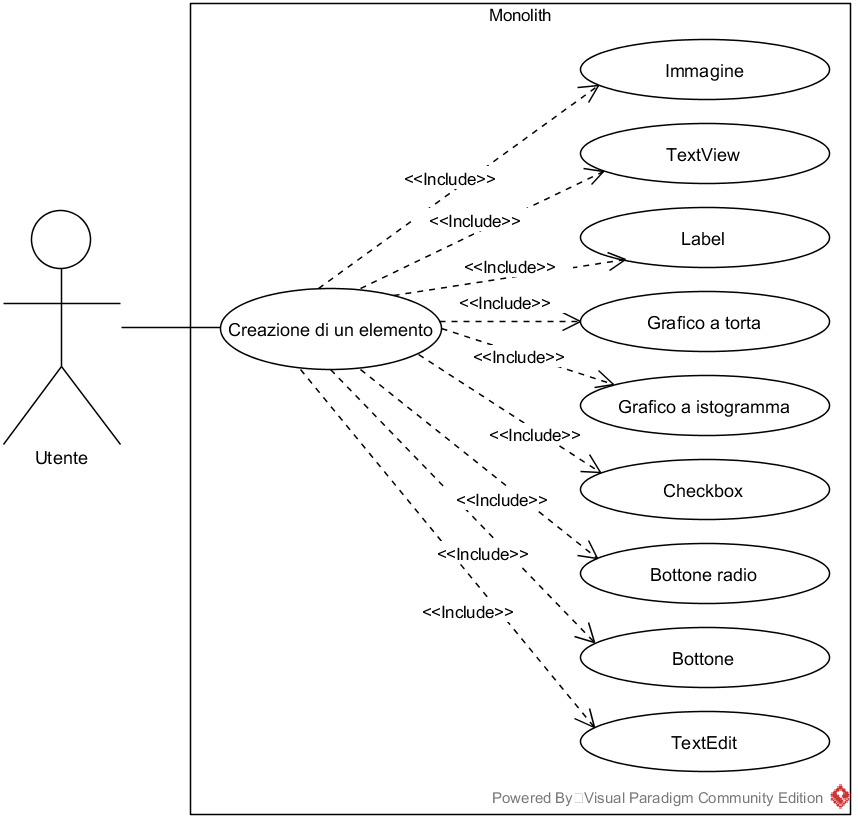
\includegraphics[width=15cm]{../../documenti/AnalisiDeiRequisiti/Diagrammi_img/creazione_elem.png}
	\caption{\UCFCaption{} Creazione di un elemento}
\end{figure}
\end{samepage}

\begin{itemize}
	\item \textbf{Attori:}
	\\Utilizzatore del framework.
	\item \textbf{Scopo e descrizione:} 
	\\Costruzione di un elemento.
	\item \textbf{Precondizioni:}
	\begin{itemize}
		\item Avere già istanziato una bubble generica;
		\item Disporre di tutte le risorse necessarie a creare l'elemento.
	\end{itemize}
	\item \textbf{Flusso principale degli eventi:}
	\begin{itemize}
		\item L'utilizzatore del framework crea un elemento di tipo Immagine \ref{UC1.25};
		\item L'utilizzatore del framework crea un elemento di tipo TextView \ref{UC1.26};
		\item L'utilizzatore del framework crea un elemento di tipo Label \ref{UC1.27};
		\item L'utilizzatore del framework crea un elemento di tipo Grafico a torta \ref{UC1.28};
		\item L'utilizzatore del framework crea un elemento di tipo Grafico a istogramma \ref{UC1.29};
		\item L'utilizzatore del framework crea un elemento di tipo Checkbox \ref{UC1.30};
		\item L'utilizzatore del framework crea un elemento di tipo Bottone radio \ref{UC1.31};
		\item L'utilizzatore del framework crea un elemento di tipo Bottone \ref{UC1.32};
		\item L'utilizzatore del framework crea un elemento di tipo TextEdit \ref{UC1.33}; 
	\end{itemize}
	\item \textbf{Post-condizione:}
	\\È stato creato un elemento.
\end{itemize}

\begin{samepage}
\UCFF{Immagine}{UC1.25}
\nopagebreak
\begin{figure}[H]
	\centering
	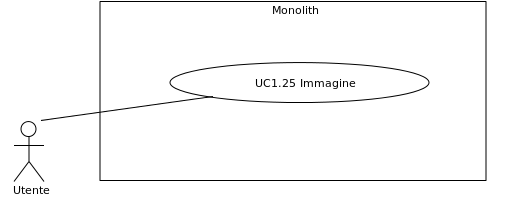
\includegraphics[width=15cm]{../../documenti/AnalisiDeiRequisiti/Diagrammi_img/uc1_25.png}
	\caption{\UCFFCaption{} Immagine}
\end{figure}
\end{samepage}

\begin{itemize}
	\item \textbf{Attori:}
	\\Utilizzatore del framework.
	\item \textbf{Scopo e descrizione:} 
	\\L'utilizzatore del framework può creare un elemento immagine.
	\item \textbf{Precondizioni:}
	\begin{itemize}
		\item Avere già istanziato una bubble generica;
		\item Avere un'immagine di cui fare la preview.
	\end{itemize}
	\item \textbf{Flusso principale degli eventi:}
	\\L'utilizzatore del framework crea un elemento immagine.
	\item \textbf{Post-condizione:}
	\\È stato creato un elemento immagine.
\end{itemize}

\begin{samepage}
\UCFF{TextView}{UC1.26}
\nopagebreak
\begin{figure}[H]
	\centering
	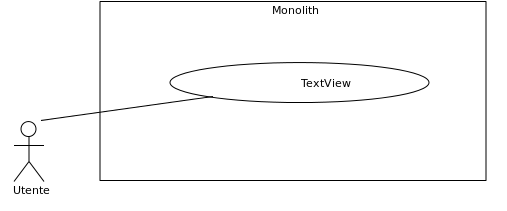
\includegraphics[width=15cm]{../../documenti/AnalisiDeiRequisiti/Diagrammi_img/uc1_26.png}
	\caption{\UCFFCaption{} TextView}
\end{figure}
\end{samepage}

\begin{itemize}
	\item \textbf{Attori:}
	\\Utilizzatore del framework.
	\item \textbf{Scopo e descrizione:} 
	\\L'utilizzatore del framework può creare un elemento \glossario{TextView}.
	\item \textbf{Precondizioni:}
	\begin{itemize}
		\item Avere già istanziato una bubble generica;
		\item Avere un testo da visualizzare.
	\end{itemize}
	\item \textbf{Flusso principale degli eventi:}
	\\L'utilizzatore del framework crea l'elemento TextView specificando il testo da includere.
	\item \textbf{Post-condizione:}
	\\È stato creato un elemento TextView.
\end{itemize}

\begin{samepage}
\UCFF{Label}{UC1.27}
\nopagebreak
\begin{figure}[H]
	\centering
	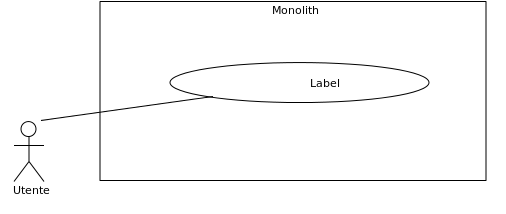
\includegraphics[width=15cm]{../../documenti/AnalisiDeiRequisiti/Diagrammi_img/uc1_27.png}
	\caption{\UCFFCaption{} Label}
\end{figure}
\end{samepage}

\begin{itemize}
	\item \textbf{Attori:}
	\\Utilizzatore del framework.
	\item \textbf{Scopo e descrizione:} 
	\\L'utilizzatore del framework può creare un elemento \glossario{label}.
	\item \textbf{Precondizioni:}
	\begin{itemize}
		\item Avere già istanziato una bubble generica;
		\item Avere un testo da visualizzare.
	\end{itemize}
	\item \textbf{Flusso principale degli eventi:}
	\\L'utilizzatore del framework crea l'elemento label specificando il testo da includere.
	\item \textbf{Post-condizione:}
	\\È stato creato un elemento label.
\end{itemize}

\begin{samepage}
\UCFF{Grafico a torta}{UC1.28}
\nopagebreak
\begin{figure}[H]
	\centering
	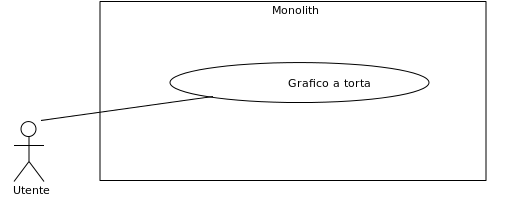
\includegraphics[width=15cm]{../../documenti/AnalisiDeiRequisiti/Diagrammi_img/uc1_28.png}
	\caption{\UCFFCaption{} Grafico a torta}
\end{figure}
\end{samepage}

\begin{itemize}
	\item \textbf{Attori:}
	\\Utilizzatore del framework.
	\item \textbf{Scopo e descrizione:} 
	\\L'utilizzatore del framework può creare un elemento "grafico a torta".
	\item \textbf{Precondizioni:}
	\begin{itemize}
		\item Avere già istanziato una bubble generica;
		\item Essere in possesso dei dati che si desidera visualizzare nel grafico.
	\end{itemize}
	\item \textbf{Flusso principale degli eventi:}
	\\L'utilizzatore del framework crea l'elemento specificando i dati da rappresentare nel grafico a torta.
	\item \textbf{Post-condizione:}
	\\È stato creato un elemento "grafico a torta".
\end{itemize}

\begin{samepage}
\UCFF{Grafico a istogramma}{UC1.29}
\nopagebreak
\begin{figure}[H]
	\centering
	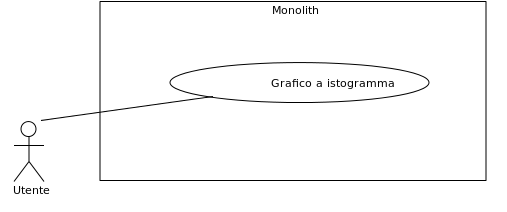
\includegraphics[width=15cm]{../../documenti/AnalisiDeiRequisiti/Diagrammi_img/uc1_29.png}
	\caption{\UCFFCaption{} Grafico a istogramma}
\end{figure}
\end{samepage}

\begin{itemize}
	\item \textbf{Attori:}
	\\Utilizzatore del framework.
	\item \textbf{Scopo e descrizione:} 
	\\L'utilizzatore del framework può creare un elemento "grafico a istogramma".
	\item \textbf{Precondizioni:}
	\begin{itemize}
		\item Avere già istanziato una bubble generica;
		\item Essere in possesso dei dati che si desidera visualizzare nel grafico.
	\end{itemize}
	\item \textbf{Flusso principale degli eventi:}
	\\L'utilizzatore del framework crea l'elemento specificando i dati da rappresentare nel grafico a istogramma.
	\item \textbf{Post-condizione:}
	\\È stato creato un elemento "grafico a istogramma".
\end{itemize}

\begin{samepage}
\UCFF{Checkbox}{UC1.30}
\nopagebreak
\begin{figure}[H]
	\centering
	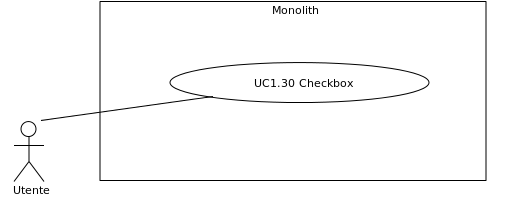
\includegraphics[width=15cm]{../../documenti/AnalisiDeiRequisiti/Diagrammi_img/uc1_30.png}
	\caption{\UCFFCaption{} Checkbox}
\end{figure}
\end{samepage}

\begin{itemize}
	\item \textbf{Attori:}
	\\Utilizzatore del framework.
	\item \textbf{Scopo e descrizione:} 
	\\L'utilizzatore del framework può creare un elemento \glossario{checkbox}.
	\item \textbf{Precondizioni:}
	\begin{itemize}
		\item Avere già istanziato una bubble generica.
	\end{itemize}
	\item \textbf{Flusso principale degli eventi:}
	\\L'utilizzatore del framework crea l'elemento checkbox.
	\item \textbf{Post-condizione:}
	\\È stato creato l'elemento checkbox.
\end{itemize}

\begin{samepage}
\UCFF{Bottone Radio}{UC1.31}
\nopagebreak
\begin{figure}[H]
	\centering
	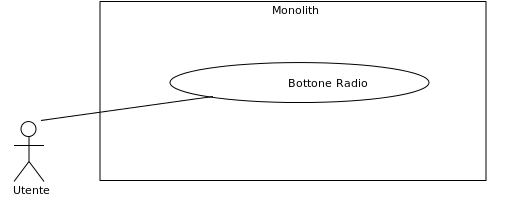
\includegraphics[width=15cm]{../../documenti/AnalisiDeiRequisiti/Diagrammi_img/uc1_31.png}
	\caption{\UCFFCaption{} Bottone Radio}
\end{figure}
\end{samepage}

\begin{itemize}
	\item \textbf{Attori:}
	\\Utilizzatore del framework.
	\item \textbf{Scopo e descrizione:} 
	\\L'utilizzatore del framework può creare un elemento \glossario{bottone radio}.
	\item \textbf{Precondizioni:}
	\begin{itemize}
		\item Avere già istanziato una bubble generica.
	\end{itemize}
	\item \textbf{Flusso principale degli eventi:}
	\\L'utilizzatore del framework crea un elemento bottone radio.
	\item \textbf{Post-condizione:}
	\\È stato creato l'elemento bottone radio.
\end{itemize}

\begin{samepage}
\UCFF{Bottone}{UC1.32}
\nopagebreak
\begin{figure}[H]
	\centering
	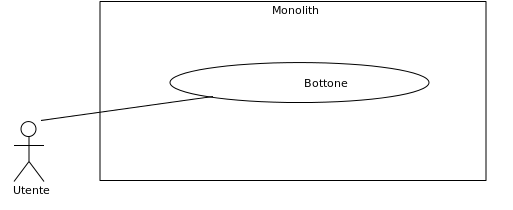
\includegraphics[width=15cm]{../../documenti/AnalisiDeiRequisiti/Diagrammi_img/uc1_32.png}
	\caption{\UCFFCaption{} Bottone}
\end{figure}
\end{samepage}

\begin{itemize}
	\item \textbf{Attori:}
	\\Utilizzatore del framework.
	\item \textbf{Scopo e descrizione:} 
	\\L'utilizzatore del framework può creare un elemento \glossario{bottone}.
	\item \textbf{Precondizioni:}
	\begin{itemize}
		\item Avere già istanziato una bubble generica;
		\item Avere la funzione da eseguire.
	\end{itemize}
	\item \textbf{Flusso principale degli eventi:}
	\\L'utilizzatore del framework crea l'elemento bottone specificando la funzione da assegnare ad esso.
	\item \textbf{Post-condizione:}
	\\È stato creato un elemento bottone
\end{itemize}

\begin{samepage}
\UCFF{TextEdit}{UC1.33}
\nopagebreak
\begin{figure}[H]
	\centering
	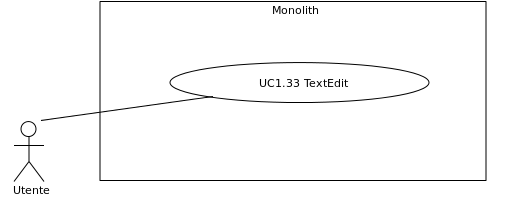
\includegraphics[width=15cm]{../../documenti/AnalisiDeiRequisiti/Diagrammi_img/uc1_33.png}
	\caption{\UCFFCaption{} TextEdit}
\end{figure}
\end{samepage}

\begin{itemize}
	\item \textbf{Attori:}
	\\Utilizzatore del framework.
	\item \textbf{Scopo e descrizione:} 
	\\L'utilizzatore del framework può creare un input testuale \glossario{TextEdit}.
	\item \textbf{Precondizioni:}
	\begin{itemize}
		\item Avere già istanziato una bubble generica.
	\end{itemize}
	\item \textbf{Flusso principale degli eventi:}
	\\L'utilizzatore del framework crea l'elemento TextEdit.
	\item \textbf{Post-condizione:}
	\\È stato creato l'elemento TextEdit.
\end{itemize}

\begin{samepage}
\UCF{Aggiunta di un elemento}{UC1.04}
\nopagebreak
\begin{figure}[H]
	\centering
	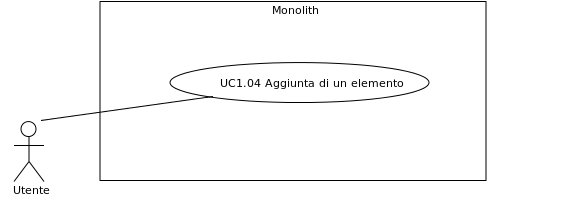
\includegraphics[width=15cm]{../../documenti/AnalisiDeiRequisiti/Diagrammi_img/uc1_04.png}
	\caption{\UCFCaption{} Aggiunta di un elemento}
\end{figure}
\end{samepage}

\begin{itemize}
	\item \textbf{Attori:}
	\\Utilizzatore del framework.
	\item \textbf{Scopo e descrizione:} 
	\\Inserire nella bubble un elemento.
	\item \textbf{Precondizioni:}
	\begin{itemize}
		\item Avere già istanziato una bubble generica;
		\item Aver istanziato un elemento.
	\end{itemize}
	\item \textbf{Flusso principale degli eventi:}
	\\L'utilizzatore invoca il metodo sulla bubble indicando l'elemento da aggiungere e il metodo lo aggiunge alla bubble.
	\item \textbf{Post-condizione:}
	\\La bubble avrà al suo interno l'elemento passato al metodo.
\end{itemize}

\begin{samepage}
\isfirsttrue
\UCC[2]{Rimozione di un elemento presente}{UC1.03.1}
\nopagebreak
\begin{figure}[H]
	\centering
	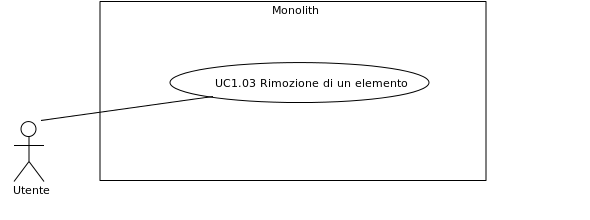
\includegraphics[width=15cm]{../../documenti/AnalisiDeiRequisiti/Diagrammi_img/uc1_03.png}
	\caption{\UCCCaption{} Rimozione di un elemento}
\end{figure}
\end{samepage}

\begin{itemize}
	\item \textbf{Attori:}
	\\Utilizzatore del framework.
	\item \textbf{Scopo e descrizione:}
	\\Rimuovere dalla bubble un \glossario{elemento}\footnote{Viene considerato elemento del framework un qualsiasi componente grafico (form, immagini, label ad esempio) o funzionale (notifiche, API).} specificato.
	\item \textbf{Precondizioni:}
	\begin{itemize}
		\item Avere già istanziato una bubble generica;
		\item La bubble possiede degli \glossario{elementi}.
	\end{itemize}
	\item \textbf{Flusso principale degli eventi:}
	\\L'utilizzatore chiama il metodo, il quale rimuove l'elemento dalla bubble.
	\item \textbf{Scenari alternativi:}
	\\L'elemento che si vuole eliminare non è presente nella bubble \ref{UC1.03.2}.
	\item \textbf{Post-condizione:}
	\\La bubble non contiene l'elemento indicato da rimuovere.
\end{itemize}

\UCC[2]{Rimozione di un elemento non presente}{UC1.03.2}

\begin{itemize}
	\item \textbf{Attori:}
	\\Utilizzatore del framework.
	\item \textbf{Scopo e descrizione:} 
	\\Rimuovere dalla bubble un elemento specificato.
	\item \textbf{Precondizioni:}
	\begin{itemize}
		\item Avere già istanziato una bubble generica;
		\item La bubble possiede degli elementi.
	\end{itemize}
	\item \textbf{Flusso principale degli eventi:}
	\\L'utilizzatore chiama il metodo, il quale, non trovando l'elemento, restituisce un messaggio di errore.
	\item \textbf{Scenari alternativi:}
	\\L'elemento è presente nella bubble \ref{UC1.03.1}.
	\item \textbf{Post-condizione:}
	\\La bubble non contiene l'elemento indicato da rimuovere e l'utilizzatore è stato avvisato della sua mancanza.
\end{itemize}

\begin{samepage}
\isfirsttrue
\UCC[2]{Modifica di un elemento presente}{UC1.05.1}
\nopagebreak
\begin{figure}[H]
	\centering
	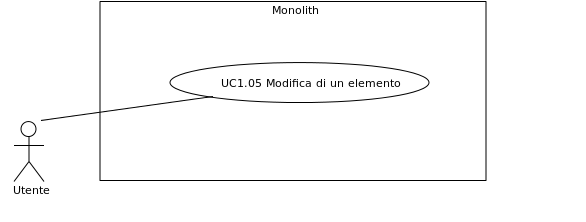
\includegraphics[width=15cm]{../../documenti/AnalisiDeiRequisiti/Diagrammi_img/uc1_05.png}
	\caption{\UCCCaption{} Modifica di un elemento}
\end{figure}
\end{samepage}

\begin{itemize}
	\item \textbf{Attori:}
	\\Utilizzatore del framework.
	\item \textbf{Scopo e descrizione:} 
	\\Modificare un elemento di una bubble.
	\item \textbf{Precondizioni:}
	\begin{itemize}
		\item Avere già istanziato una bubble generica;
		\item All'interno della bubble sono presenti degli elementi.
	\end{itemize}
	\item \textbf{Flusso principale degli eventi:}
	\\L'utilizzatore invoca il metodo sulla bubble e il metodo modifica l'elemento.
	\item \textbf{Scenari alternativi:}
	\\L'elemento che si vuole modificare non è presente nella bubble \ref{UC1.05.2}.
	\item \textbf{Post-condizione:}
	\\La bubble contiene l'elemento modificato.
\end{itemize}

\UCC[2]{Modifica di un elemento non presente}{UC1.05.2}

\begin{itemize}
	\item \textbf{Attori:}
	\\Utilizzatore del framework.
	\item \textbf{Scopo e descrizione:} 
	\\Modificare un elemento di una bubble.
	\item \textbf{Precondizioni:}
	\begin{itemize}
		\item Avere già istanziato una bubble generica;
		\item All'interno della bubble sono presenti degli elementi.
	\end{itemize}
	\item \textbf{Flusso principale degli eventi:}
	\\L'utilizzatore invoca il metodo sulla bubble e il metodo, non trovando l'elemento da modificare, lancia un messaggio di errore.
	\item \textbf{Scenari alternativi:}
	\\L'elemento è presente nella bubble \ref{UC1.05.1}.
	\item \textbf{Post-condizione:}
	\\L'utilizzatore del metodo è a conoscenza che la modifica è fallita in quanto non era presente l'elemento da modificare.
\end{itemize}

\begin{samepage}
\UCF{Creazione notifica statica}{UC1.17}
\nopagebreak
\begin{figure}[H]
	\centering
	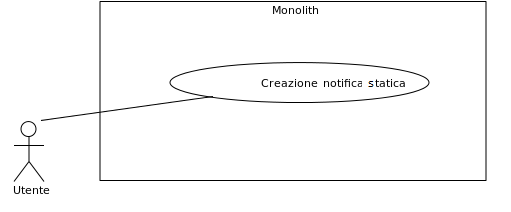
\includegraphics[width=15cm]{../../documenti/AnalisiDeiRequisiti/Diagrammi_img/uc1_17.png}
	\caption{\UCFCaption{} Creazione notifica statica}
\end{figure}
\end{samepage}

\begin{itemize}
	\item \textbf{Attori:}
	\\Utilizzatore del framework.
	\item \textbf{Scopo e descrizione:} 
	\\L'utilizzatore del framework potrà creare una notifica statica specificandone il testo.
	\item \textbf{Precondizioni:}
	\begin{itemize}
		\item Avere già istanziato una bubble generica;
		\item Essere in possesso del messaggio che si desidera notificare sotto forma di testo.
	\end{itemize}
	\item \textbf{Flusso principale degli eventi:}
	\\L'utilizzatore del framework chiama il metodo specificando il testo da visualizzare nella notifica statica.
	\item \textbf{Post-condizione:}
	\\Sul dispositivo sul quale si sta utilizzando Rocket.Chat sarà notificato il testo specificato nel metodo.
\end{itemize}

\begin{samepage}
\UCF{Visualizza notifica statica}{UC1.18}
\nopagebreak
\begin{figure}[H]
	\centering
	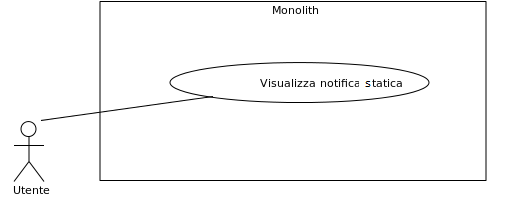
\includegraphics[width=15cm]{../../documenti/AnalisiDeiRequisiti/Diagrammi_img/uc1_18.png}
	\caption{\UCFCaption{} Visualizza notifica statica}
\end{figure}
\end{samepage}

\begin{itemize}
	\item \textbf{Attori:}
	\begin{itemize}
		\item Utilizzatore del framework;
		\item Rocket.Chat.
	\end{itemize}
	\item \textbf{Scopo e descrizione:} 
	\\L'utilizzatore del framework può far visualizzare all'utente una notifica statica che visualizzi del testo.
	\item \textbf{Precondizioni:}
	\begin{itemize}
		\item Avere già istanziato una bubble generica;
		\item Aver creato una notifica statica.
	\end{itemize}
	\item \textbf{Flusso principale degli eventi:}
	\\L'utilizzatore del framework fa visualizzare una certa notifica da lui creata.
	\item \textbf{Post-condizione:}
	\\La notifica contiene il valore del testo specificato.
\end{itemize}

\begin{samepage}
\UCF{Mostra elemento grafico}{UC1.21}
\nopagebreak
\begin{figure}[H]
	\centering
	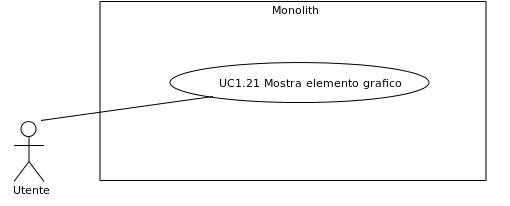
\includegraphics[width=15cm]{../../documenti/AnalisiDeiRequisiti/Diagrammi_img/uc1_21.png}
	\caption{\UCFCaption{} Mostra elemento grafico}
\end{figure}
\end{samepage}

\begin{itemize}
	\item \textbf{Attori:}
	\begin{itemize}
		\item Utilizzatore del framework;
		\item Rocket.Chat.
	\end{itemize}
	\item \textbf{Scopo e descrizione:} 
	\\L'utilizzatore del framework potrà mostrare un \glossario{elemento grafico}.\footnote{Esempi di elementi grafici sono: label, immagini, textview.}
	\item \textbf{Precondizioni:}
	\begin{itemize}
		\item Avere già istanziato una bubble generica;
		\item Avere almeno un elemento grafico nella bubble.
	\end{itemize}
	\item \textbf{Flusso principale degli eventi:}
	\\L'utilizzatore del framework chiama il metodo specificando quale elemento grafico della bubble vuole mostrare.
	\item \textbf{Post-condizione:}
	\\L'elemento grafico specificato è visibile.
\end{itemize}

\begin{samepage}
\UCF{Nascondi elemento grafico}{UC1.22}
\nopagebreak
\begin{figure}[H]
	\centering
	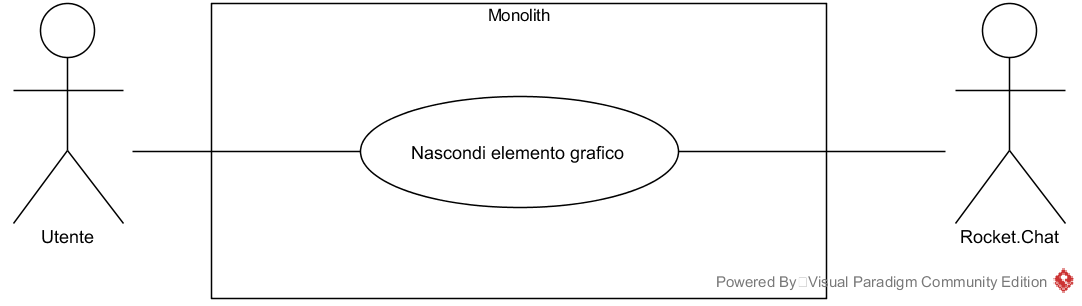
\includegraphics[width=15cm]{../../documenti/AnalisiDeiRequisiti/Diagrammi_img/uc1_22.png}
	\caption{\UCFCaption{} Nascondi elemento grafico}
\end{figure}
\end{samepage}

\begin{itemize}
	\item \textbf{Attori:}
	\begin{itemize}
		\item Utilizzatore del framework;
		\item Rocket.Chat.
	\end{itemize}
	\item \textbf{Scopo e descrizione:} 
	\\L'utilizzatore del framework potrà nascondere un elemento grafico.
	\item \textbf{Precondizioni:}
	\begin{itemize}
		\item Avere già istanziato una bubble generica;
		\item Avere almeno un elemento nella bubble.
	\end{itemize}
	\item \textbf{Flusso principale degli eventi:}
	\\L'utilizzatore del framework chiama il metodo specificando quale elemento grafico della bubble vuole nascondere.
	\item \textbf{Post-condizione:}
	\\L'elemento grafico specificato non è più visibile.
\end{itemize}

\begin{samepage}
\UCF{Imposta posizione elemento grafico}{UC1.23}
\nopagebreak
\begin{figure}[H]
	\centering
	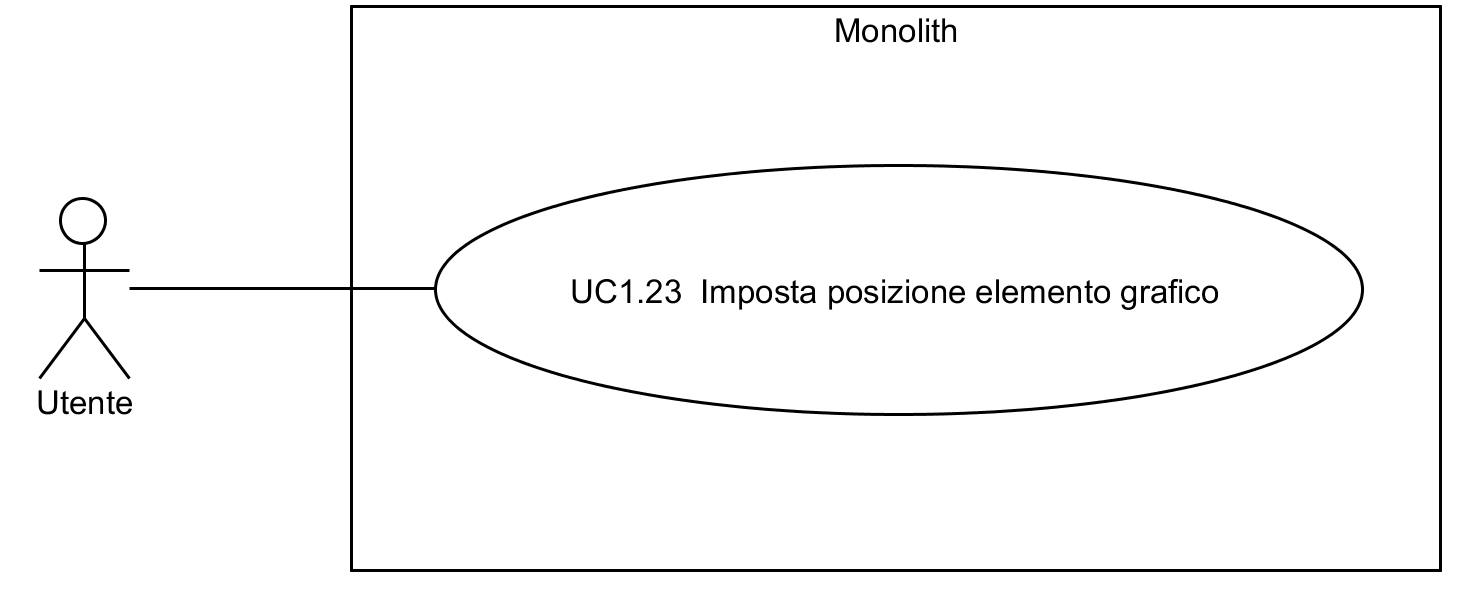
\includegraphics[width=15cm]{../../documenti/AnalisiDeiRequisiti/Diagrammi_img/uc1_23.png}
	\caption{\UCFCaption{} Imposta posizione elemento grafico}
\end{figure}
\end{samepage}

\begin{itemize}
	\item \textbf{Attori:}
	\\Utilizzatore del framework;
	\item \textbf{Scopo e descrizione:} 
	\\L'utilizzatore del framework può specificare una posizione per un elemento grafico della bubble.
	\item \textbf{Precondizioni:}
	\begin{itemize}
		\item Avere già istanziato una bubble generica;
		\item Avere almeno un componente nella bubble.
	\end{itemize}
	\item \textbf{Flusso principale degli eventi:}
	\\L'utilizzatore del framework chiama il metodo specificando la posizione e l'elemento grafico di cui vuole fissare la posizione.
	\item \textbf{Post-condizione:}
	\\L'elemento grafico specificato si trova nella posizione specificata.
\end{itemize}

\begin{samepage}
\isfirsttrue
\UCC{Cambiamento di stato della bubble su proprietà esistente}{UC1.06.1}
\nopagebreak
\begin{figure}[H]
	\centering
	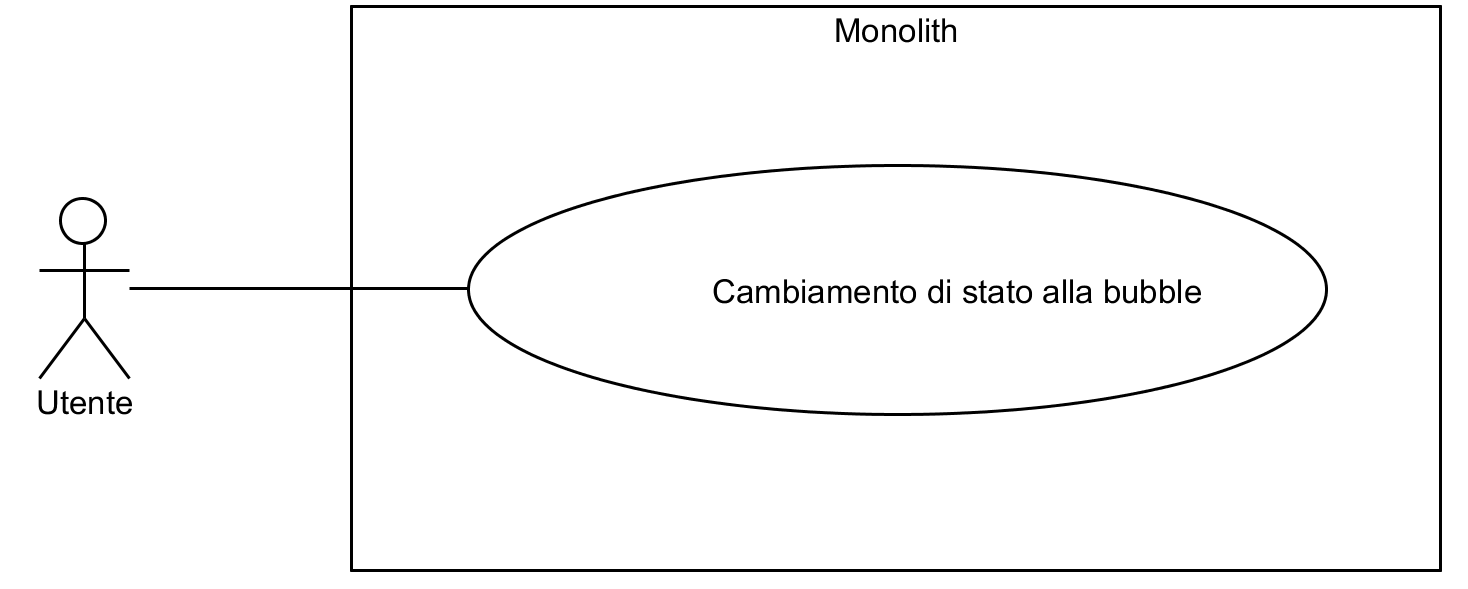
\includegraphics[width=15cm]{../../documenti/AnalisiDeiRequisiti/Diagrammi_img/uc1_06.png}
	\caption{\UCCCaption{} Cambiamento di stato della bubble}
\end{figure}
\end{samepage}

\begin{itemize}
	\item \textbf{Attori:}
	\\Utilizzatore del framework.
	\item \textbf{Scopo e descrizione:} 
	\\Modificare lo specifico stato della bubble.
	\item \textbf{Precondizioni:}
	\begin{itemize}
		\item Avere già istanziato una bubble generica.
	\end{itemize}
	\item \textbf{Flusso principale degli eventi:}
	\\L'utilizzatore invoca il metodo sulla bubble indicando il nuovo stato e il metodo esegue la modifica.
	\item \textbf{Scenari alternativi:}
	\\L'oggetto che si sta cercando di modificare non ha la proprietà cercata \ref{UC1.06.2}.
	\item \textbf{Post-condizione:}
	\\L'oggetto è stato modificato.
\end{itemize}

\UCC{Cambiamento di stato della bubble su proprietà non esistente}{UC1.06.2}

\begin{itemize}
	\item \textbf{Attori:}
	\\Utilizzatore del framework.
	\item \textbf{Scopo e descrizione:} 
	\\Modificare lo specifico stato della bubble.
	\item \textbf{Precondizioni:}
	\begin{itemize}
		\item Avere già istanziato una bubble generica.
	\end{itemize}
	\item \textbf{Flusso principale degli eventi:}
	\\L'utilizzatore invoca il metodo sulla bubble indicando il nuovo stato e il metodo, non trovando la proprietà cercata, restituisce un messaggio di errore.
	\item \textbf{Scenari alternativi:}
	\\L'oggetto che si sta cercando di modificare ha la proprietà cercata \ref{UC1.06.1}.
	\item \textbf{Post-condizione:}
	\\L'oggetto non è stato modificato.
\end{itemize}

\begin{samepage}
\isfirsttrue
\UCC{Chiamata API esterne disponibili}{UC1.07.1}
\nopagebreak
\begin{figure}[H]
	\centering
	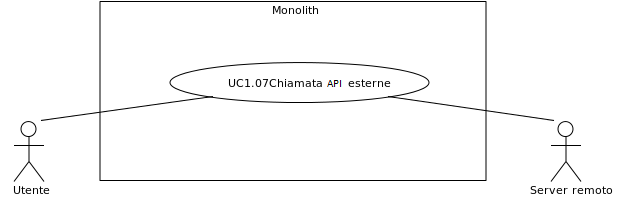
\includegraphics[width=15cm]{../../documenti/AnalisiDeiRequisiti/Diagrammi_img/uc1_07.png}
	\caption{\UCCCaption{} Chiamata API esterne}
\end{figure}
\end{samepage}

\begin{itemize}
	\item \textbf{Attori:}
	\\Utilizzatore del framework.
	\item \textbf{Scopo e descrizione:} 
	\\Ottenere il risultato dell'interrogazione di un servizio esterno al framework tramite chiamata di \glossario{API}.
	\item \textbf{Precondizioni:}
	\begin{itemize}
		\item Avere già istanziato una bubble generica;
		\item Conoscere l'URL del servizio desiderato.
	\end{itemize}
	\item \textbf{Flusso principale degli eventi:}
	\\Il metodo prende l'indirizzo del servizio e ritorna in formato JSON il risultato della chiamata.
	\item \textbf{Scenari alternativi:}
	\\Il servizio che si sta cercando di contattare non è disponibile \ref{UC1.07.2}.
	\item \textbf{Post-condizione:}
	\\All'interno della logica della bubble è utilizzabile il risultato della consultazione del servizio.
\end{itemize}

\UCC{Chiamata API esterne non disponibili}{UC1.07.2}

\begin{itemize}
	\item \textbf{Attori:}
	\\Utilizzatore del framework.
	\item \textbf{Scopo e descrizione:} 
	\\Ottenere il risultato dell'interrogazione di un servizio esterno al framework tramite chiamata di API.
	\item \textbf{Precondizioni:}
	\begin{itemize}
		\item Avere già istanziato una bubble generica;
		\item Conoscere l'URL del servizio desiderato.
	\end{itemize}
	\item \textbf{Flusso principale degli eventi:}
	\\Il metodo prende l'indirizzo del servizio e, non trovandolo disponibile, ritorna un messaggio di errore.
	\item \textbf{Scenari alternativi:}
	\\Il servizio che si sta cercando di contattare è disponibile \ref{UC1.07.1}.
	\item \textbf{Post-condizione:}
	\\L'utilizzatore del metodo è stato avvisato della non disponibilità del servizio.
\end{itemize}

\UC{Controllo sul JSON}{UC1.12}

\begin{figure}[H]
	\centering
	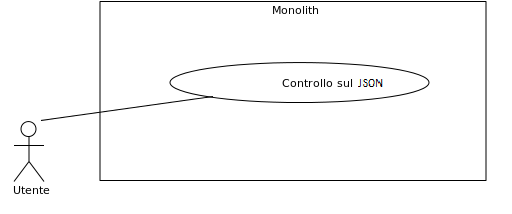
\includegraphics[width=15cm]{../../documenti/AnalisiDeiRequisiti/Diagrammi_img/uc1_12.png}
	\caption{\UCCaption{} Controllo sul JSON}
\end{figure}

\begin{itemize}
	\item \textbf{Attori:}
	\\Utilizzatore del framework.
	\item \textbf{Scopo e descrizione:} 
	\\Verificare che la struttura di un oggetto JSON sia compatibile con lo schema fornito.
	\item \textbf{Precondizioni:}
	\begin{itemize}
		\item Avere già istanziato una bubble generica;
		\item Avere un oggetto JSON da validare;
		\item Avere lo schema attraverso cui validare l'oggetto JSON.
	\end{itemize}
	\item \textbf{Flusso principale degli eventi:}
	\\Alla chiamata del metodo viene specificato il JSON da verificare e lo schema di dati rispetto al quale validare tale oggetto. Il metodo poi si occupa della validazione.
	\item \textbf{Post-condizione:}
	\\È noto se l'oggetto JSON è compatibile con la struttura indicata.
\end{itemize}

\UC{Settare le impostazioni della bubble}{UCimpostazioni}
\begin{figure}[H]
	\centering
	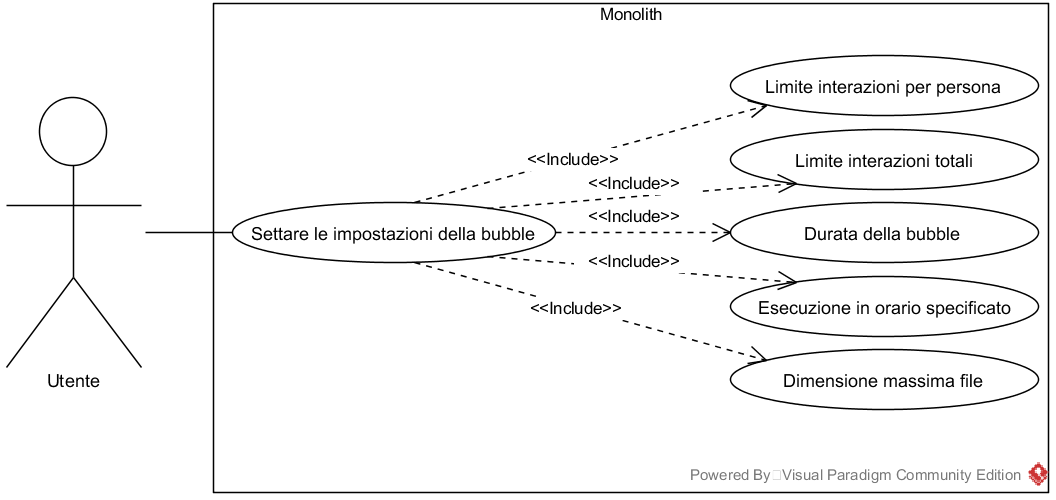
\includegraphics[width=15cm]{../../documenti/AnalisiDeiRequisiti/Diagrammi_img/Impostazioni.png}
	\caption{\UCCaption{} Settare le impostazioni della bubble}
\end{figure}

\begin{itemize}
	\item \textbf{Attori:}
	\\Utilizzatore del framework.
	\item \textbf{Scopo e descrizione:} 
	\\Modificare le impostazioni della bubble per adattarle allo scopo della stessa.
	\item \textbf{Precondizioni:}
	\begin{itemize}
		\item Avere già istanziato una bubble generica;
	\end{itemize}
	\item \textbf{Flusso principale degli eventi:}
	\begin{itemize}
		\item L'utente imposta un limite di interazioni per persona \ref{UC1.08};
		\item L'utente imposta un limite di interazioni totali \ref{UC1.09};
		\item L'utente imposta la durata della bubble \ref{UC1.13};
		\item L'utente specifica l'orario di esecuzione \ref{UC1.16};
		\item L'utente imposta una dimensione massima per i file \ref{}.
	\end{itemize}
	\item \textbf{Post-condizione:}
	\\La bubble è stata configurata con le impostazioni definite.
\end{itemize}

\begin{samepage}
\UCF{Limite interazioni per persona}{UC1.08}
\nopagebreak
\begin{figure}[H]
	\centering
	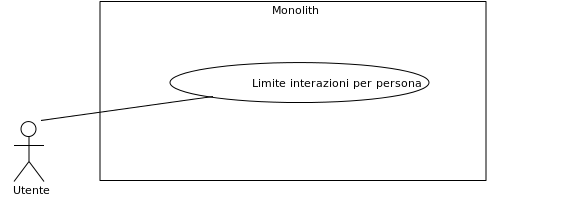
\includegraphics[width=15cm]{../../documenti/AnalisiDeiRequisiti/Diagrammi_img/uc1_08.png}
	\caption{\UCFCaption{} Limite interazioni per persona}
\end{figure}
\end{samepage}

\begin{itemize}
	\item \textbf{Attori:}
	\\Utilizzatore del framework.
	\item \textbf{Scopo e descrizione:} 
	\\Porre un limite superiore al numero delle interazioni che un utente di Rocket.Chat può avere con una stessa bubble.
	\item \textbf{Precondizioni:}
	\begin{itemize}
		\item Avere già istanziato una bubble generica;
		\item Avere almeno un \glossario{elemento di input} all'interno della bubble.
	\end{itemize}
	\item \textbf{Flusso principale degli eventi:}
	\\Alla chiamata del metodo viene specificato il numero massimo di interazioni possibili per una persona con una singola istanza della bubble.
	\item \textbf{Post-condizione:}
	\\Il singolo utilizzatore della bubble come utente di Rocket.Chat non potrà interagire con la stessa istanza della bubble più volte di quelle specificate.
\end{itemize}

\begin{samepage}
\UCF{Limite interazioni totali}{UC1.09}
\nopagebreak
\begin{figure}[H]
	\centering
	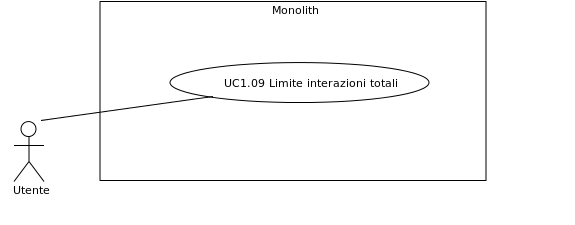
\includegraphics[width=15cm]{../../documenti/AnalisiDeiRequisiti/Diagrammi_img/uc1_09.png}
	\caption{\UCFCaption{} Limite interazioni totali}
\end{figure}
\end{samepage}

\begin{itemize}
	\item \textbf{Attori:}
	\\Utilizzatore del framework.
	\item \textbf{Scopo e descrizione:} 
	\\Porre un limite superiore al numero delle interazioni che tutti gli utenti possono avere con una stessa istanza della bubble.
	\item \textbf{Precondizioni:}
	\begin{itemize}
		\item Avere già istanziato una bubble generica;
		\item Avere almeno un elemento di input all'interno della bubble.
	\end{itemize}
	\item \textbf{Flusso principale degli eventi:}
	\\Alla chiamata del metodo viene specificato il numero massimo di interazioni possibili per l'istanza della bubble.
	\item \textbf{Post-condizione:}
	\\La singola istanza della bubble ha un numero massimo di interazioni possibili condiviso tra tutti i suoi utenti. 
\end{itemize}

\begin{samepage}
\UCF{Durata della bubble}{UC1.13}
\nopagebreak
\begin{figure}[H]
	\centering
	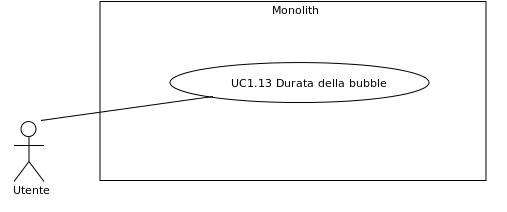
\includegraphics[width=15cm]{../../documenti/AnalisiDeiRequisiti/Diagrammi_img/uc1_13.png}
	\caption{\UCFCaption{} Durata della bubble}
\end{figure}
\end{samepage}

\begin{itemize}
	\item \textbf{Attori:}
	\\Utilizzatore del framework.
	\item \textbf{Scopo e descrizione:} 
	\\Dare la possibilità all'utilizzatore del framework di impostare un limite temporale entro il quale la bubble smetterà di essere attiva.
	\item \textbf{Precondizioni:}
	\begin{itemize}
		\item Avere già istanziato una bubble generica.
	\end{itemize}
	\item \textbf{Flusso principale degli eventi:}
	\\Alla chiamata del metodo viene specificato il tempo per il quale la bubble sarà attiva.
	\item \textbf{Post-condizione:}
	\\Al termine del periodo di tempo specificato dal metodo verrà invocata la sua terminazione secondo quanto specificato nel caso d'uso \ref{UC1.19} termina bubble.
\end{itemize}

\begin{samepage}
\UCF{Esecuzione in orario specificato}{UC1.16}
\nopagebreak
\begin{figure}[H]
	\centering
	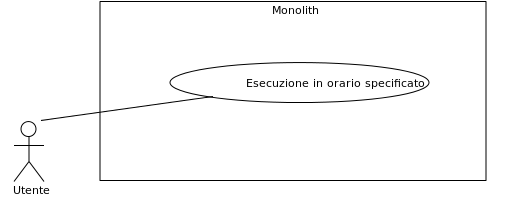
\includegraphics[width=15cm]{../../documenti/AnalisiDeiRequisiti/Diagrammi_img/uc1_16.png}
	\caption{\UCFCaption{} Esecuzione in orario specificato}
\end{figure}
\end{samepage}

\begin{itemize}
	\item \textbf{Attori:}
	\begin{itemize}
		\item Utilizzatore del framework;
		\item Rocket.Chat.
	\end{itemize}
	\item \textbf{Scopo e descrizione:} 
	\\L'utilizzatore del framework può fornire un orario per l'esecuzione della funzionalità della bubble.
	\item \textbf{Precondizioni:}
	\begin{itemize}
		\item Avere già istanziato una bubble generica;
		\item Avere la funzione di callback che si desidera eseguire all'orario specificato.
	\end{itemize}
	\item \textbf{Flusso principale degli eventi:}
	\\Alla chiamata del metodo viene specificato l'orario di esecuzione della specifica funzionalità della bubble.
	\item \textbf{Post-condizione:}
	\\Nell'orario stabilito viene eseguita la funzionalità della bubble all'interno di Rocket.Chat.
\end{itemize}

\begin{samepage}
\UCF{Dimensione massima del file}{UC1.11}
\nopagebreak
\begin{figure}[H]
	\centering
	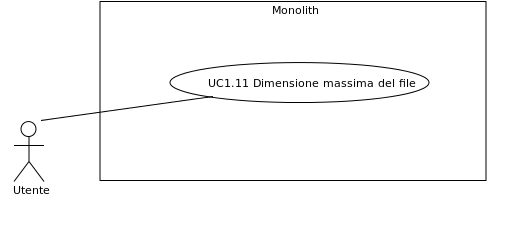
\includegraphics[width=15cm]{../../documenti/AnalisiDeiRequisiti/Diagrammi_img/uc1_11.png}
	\caption{\UCFCaption{} Dimensione massima del file}
\end{figure}
\end{samepage}

\begin{itemize}
	\item \textbf{Attori:}
	\\Utilizzatore del framework.
	\item \textbf{Scopo e descrizione:} 
	\\Verificare che la dimensione dei file caricati in input sia minore o uguale a quella specificata.
	\item \textbf{Precondizioni:}
	\begin{itemize}
		\item Avere già istanziato una bubble generica;
		\item Avere almeno un elemento di input all'interno della bubble.
	\end{itemize}
	\item \textbf{Flusso principale degli eventi:}
	\\Alla chiamata del metodo viene specificata la dimensione massima accettata per i file di input.
	\item \textbf{Post-condizione:}
	\\È stata impostata una dimensione massima per i file allegabili.
\end{itemize}

\UC{Match con espressione regolare}{UC1.10}

\begin{figure}[H]
	\centering
	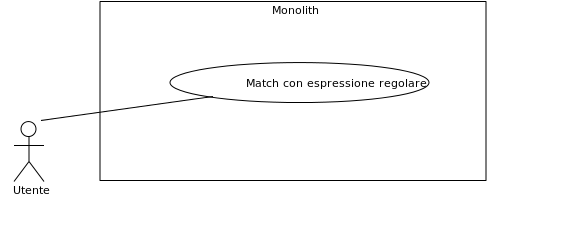
\includegraphics[width=15cm]{../../documenti/AnalisiDeiRequisiti/Diagrammi_img/uc1_10.png}
	\caption{\UCCaption{} Match con espressione regolare}
\end{figure}

\begin{itemize}
	\item \textbf{Attori:}
	\\Utilizzatore del framework.
	\item \textbf{Scopo e descrizione:} 
	\\Verificare che l'input testuale di una bubble sia compatibile con un'espressione regolare data.
	\item \textbf{Precondizioni:}
	\begin{itemize}
		\item Avere già istanziato una bubble generica;
		\item Avere almeno un elemento di input all'interno della bubble.
	\end{itemize}
	\item \textbf{Flusso principale degli eventi:}
	\\Alla chiamata del metodo viene specificato l'elemento da verificare e l'espressione regolare in base a cui controllarlo.
	\item \textbf{Post-condizione:}
	\\È noto se l'input della bubble è corretto secondo l'espressione regolare.
\end{itemize}

\UC{Lista utenti partecipanti}{UC1.14}

\begin{figure}[H]
	\centering
	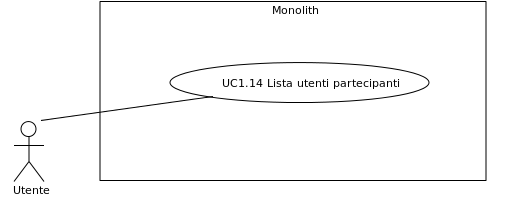
\includegraphics[width=15cm]{../../documenti/AnalisiDeiRequisiti/Diagrammi_img/uc1_14.png}
	\caption{\UCCaption{} Lista utenti partecipanti}
\end{figure}

\begin{itemize}
	\item \textbf{Attori:}
	\\Utilizzatore del framework.
	\item \textbf{Scopo e descrizione:} 
	\\Possibilità di visualizzare gli utilizzatori correnti della bubble.
	\item \textbf{Precondizioni:}
	\begin{itemize}
		\item Avere già istanziato una bubble generica.
	\end{itemize}
	\item \textbf{Flusso principale degli eventi:}
	\\Alla chiamata del metodo viene specificato l'elenco degli utilizzatori correnti della bubble.
	\item \textbf{Post-condizione:}
	\\Viene restituita una lista di utilizzatori della bubble.
\end{itemize}

\begin{samepage}
\UCC{Storico interazioni con la bubble per utente presente}{UC1.15.1}
\nopagebreak
\begin{figure}[H]
	\centering
	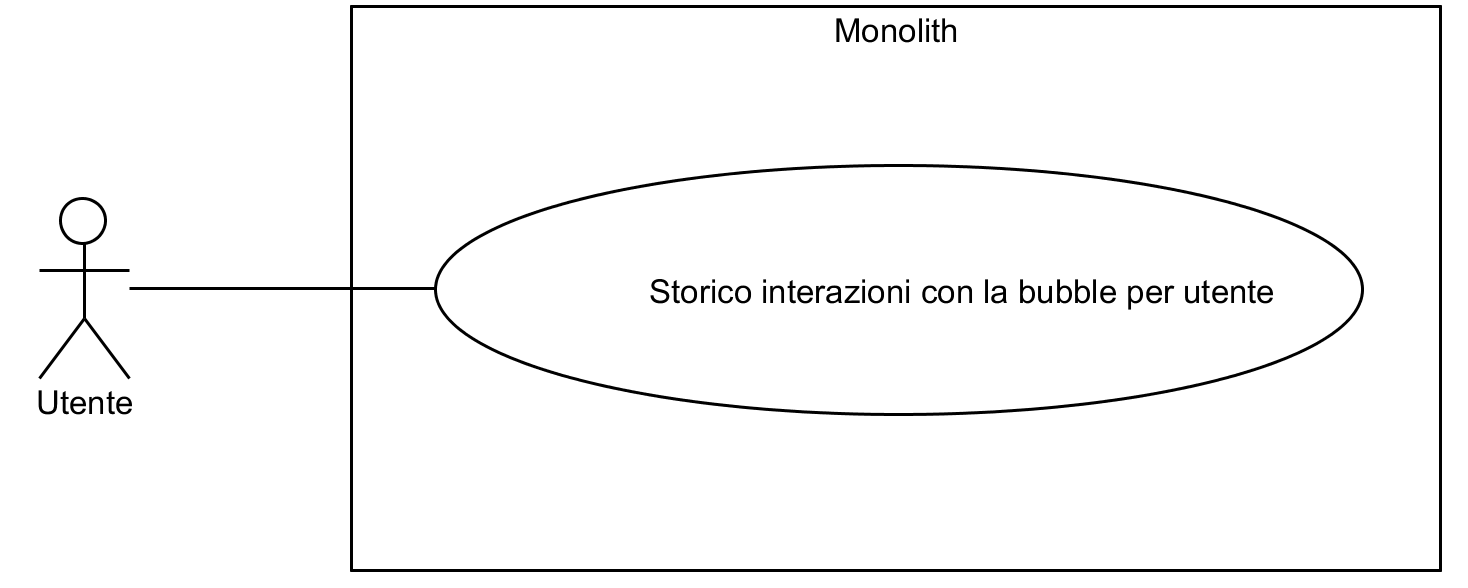
\includegraphics[width=15cm]{../../documenti/AnalisiDeiRequisiti/Diagrammi_img/uc1_15.png}
	\caption{\UCCCaption{} Storico interazioni con la bubble per utente}
\end{figure}
\end{samepage}

\begin{itemize}
	\item \textbf{Attori:}
	\\Utilizzatore del framework.
	\item \textbf{Scopo e descrizione:} 
	\\Dare la possibilità all'utilizzatore del framework di consultare lo storico delle interazioni che un singolo utente ha avuto con la bubble.
	\item \textbf{Precondizioni:}
	\begin{itemize}
		\item Avere già istanziato una bubble generica;
		\item Avere elementi di input all'interno della bubble.
	\end{itemize}
	\item \textbf{Flusso principale degli eventi:}
	\\Alla chiamata del metodo viene specificato l'utente di cui si è interessati a conoscere lo storico delle interazioni.
	\item \textbf{Scenari alternativi:}
	\\Non è presente l'utente specificato all'interno della conversazione \ref{UC1.15.2}.
	\item \textbf{Post-condizione:}
	\\L'informazione relativa allo storico delle interazioni di un singolo utente con la bubble è noto all'interno della bubble stessa.
\end{itemize}

\UCC{Storico interazioni con la bubble per utente non presente}{UC1.15.2}

\begin{itemize}
	\item \textbf{Attori:}
	\\Utilizzatore del framework.
	\item \textbf{Scopo e descrizione:} 
	\\Dare la possibilità all'utilizzatore del framework di consultare lo storico delle interazioni che un singolo utente ha avuto con la bubble.
	\item \textbf{Precondizioni:}
	\begin{itemize}
		\item Avere già istanziato una bubble generica;
		\item Avere elementi di input all'interno della bubble.
	\end{itemize}
	\item \textbf{Flusso principale degli eventi:}
	\\Alla chiamata del metodo viene specificato l'utente di cui si è interessati a conoscere lo storico delle interazioni e il metodo, non trovando l'utente, restituisce un messaggio di errore.
	\item \textbf{Scenari alternativi:}
	\\È presente l'utente specificato all'interno della conversazione \ref{UC1.15.1}.
	\item \textbf{Post-condizione:}
	\\L'utilizzatore del metodo ha ricevuto un messaggio di errore che lo avvisa dell'assenza all'interno della conversazione dell'utente di cui aveva richiesto lo storico.
\end{itemize}

\begin{samepage}
\isfirsttrue
\UCC{Converti in PDF}{UC1.20.1}
\nopagebreak
\begin{figure}[H]
	\centering
	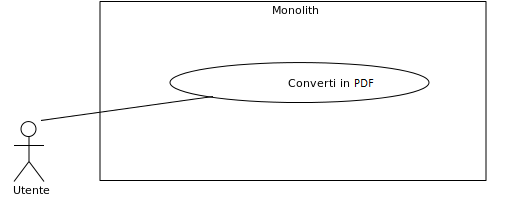
\includegraphics[width=15cm]{../../documenti/AnalisiDeiRequisiti/Diagrammi_img/uc1_20.png}
	\caption{\UCCCaption{} Converti in PDF}
\end{figure}
\end{samepage}

\begin{itemize}
	\item \textbf{Attori:}
	\\Utilizzatore del framework.
	\item \textbf{Scopo e descrizione:} 
	\\L'utilizzatore del framework potrà convertire il testo specificato in un \glossario{PDF}.
	\item \textbf{Precondizioni:}
	\begin{itemize}
		\item Avere già istanziato una bubble generica;
		\item Possedere il testo da convertire in formato PDF;
		\item Conoscere il percorso in cui si desidera che il file sia salvato.
	\end{itemize}
	\item \textbf{Flusso principale degli eventi:}
	\\L'utilizzatore del framework chiama il metodo specificando il testo da convertire in PDF e il percorso in cui si desidera salvare il file.
	\item \textbf{Scenari alternativi:}
	\\Il salvataggio del file PDF non ha successo \ref{UC1.20.2}.
	\item \textbf{Post-condizione:}
	\\Un file PDF è stato creato nella posizione corretta e contiene il testo specificato.
\end{itemize}

\UCC{Conversione in PDF fallita}{UC1.20.2}

\begin{itemize}
	\item \textbf{Attori:}
	\\Utilizzatore del framework.
	\item \textbf{Scopo e descrizione:} 
	\\L'utilizzatore del framework potrà convertire il testo specificato in un PDF.
	\item \textbf{Precondizioni:}
	\begin{itemize}
		\item Avere già istanziato una bubble generica;
		\item Possedere il testo da convertire in formato PDF;
		\item Conoscere il percorso in cui si desidera che il file sia salvato.
	\end{itemize}
	\item \textbf{Flusso principale degli eventi:}
	\\L'utilizzatore del framework chiama il metodo specificando il testo da convertire in PDF e il percorso in cui si desidera salvare il file, ma il salvataggio non avviene e l'utilizzatore del framework visualizza un messaggio d'errore.
	\item \textbf{Scenari alternativi:}
	\\Il salvataggio del file PDF ha successo \ref{UC1.20.2}.
	\item \textbf{Post-condizione:}
	\\L'utilizzatore del metodo ha ricevuto un messaggio di errore che lo avvisa che il file PDF non è stato salvato.
\end{itemize}

\begin{samepage}
\isfirsttrue
\UCC{File output}{UC1.24.1}
\nopagebreak
\begin{figure}[H]
	\centering
	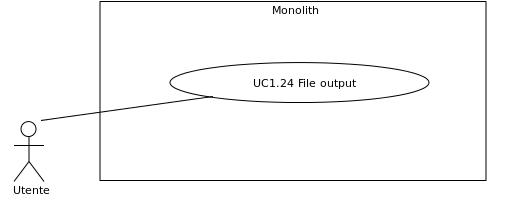
\includegraphics[width=15cm]{../../documenti/AnalisiDeiRequisiti/Diagrammi_img/uc1_24.png}
	\caption{\UCCCaption{} File output}
\end{figure}
\end{samepage}

\begin{itemize}
	\item \textbf{Attori:}
	\\Utilizzatore del framework.
	\item \textbf{Scopo e descrizione:} 
	\\L'utilizzatore del framework può salvare l'output della bubble in un file.
	\item \textbf{Precondizioni:}
	\begin{itemize}
		\item Avere già istanziato una bubble generica;
		\item Avere almeno un elemento nella bubble.
	\end{itemize}
	\item \textbf{Flusso principale degli eventi:}
	\\L'utilizzatore del framework chiama il metodo che specifica che l'output della bubble sia un file e le informazioni da salvare in esso.
	\item \textbf{Scenari alternativi:}
	\\Il salvataggio del file non ha successo, in tale caso verrà notificata la condizione anomala con un messaggio d'errore \ref{UC1.24.2}.
	\item \textbf{Post-condizione:}
	\\Verrà generato un file contenente l'informazione desiderata.
\end{itemize}

\UCC{Errore File output}{UC1.24.2}

\begin{itemize}
	\item \textbf{Attori:}
	\\Utilizzatore del framework.
	\item \textbf{Scopo e descrizione:} 
	\\L'utilizzatore del framework può salvare l'output della bubble in un file, il salvataggio non va a buon fine e viene generato un messaggio d'errore.
	\item \textbf{Precondizioni:}
	\begin{itemize}
		\item Avere già istanziato una bubble generica;
		\item Avere delle informazioni da esportare.
	\end{itemize}
	\item \textbf{Flusso principale degli eventi:}
	\\L'utilizzatore del framework chiama il metodo che specifica che l'output della bubble sia un file e le informazioni da salvare in esso, il salvataggio non va a buon fine e viene generato un messaggio d'errore.
	\item \textbf{Scenari alternativi:}
	\\Il salvataggio del file ha successo \ref{UC1.24.1}.
	\item \textbf{Post-condizione:}
	\\Viene generato un messaggio d'errore.
\end{itemize}

\UC{File input}{UC1.34}

\begin{figure}[H]
	\centering
	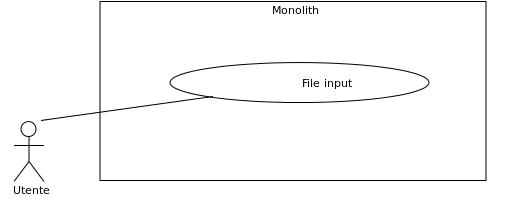
\includegraphics[width=15cm]{../../documenti/AnalisiDeiRequisiti/Diagrammi_img/uc1_34.png}
	\caption{\UCCaption{} File input}
\end{figure}

\begin{itemize}
	\item \textbf{Attori:}
	\\Utilizzatore del framework.
	\item \textbf{Scopo e descrizione:} 
	\\L'utilizzatore del framework può richiedere l'input di un file.
	\item \textbf{Precondizioni:}
	\begin{itemize}
		\item Avere già istanziato una bubble generica.
	\end{itemize}
	\item \textbf{Flusso principale degli eventi:}
	\\L'utilizzatore del framework chiama il metodo che restituisce il file in input.
	\item \textbf{Post-condizione:}
	\\Il file è stato caricato e passato alla bubble.
\end{itemize}

\UC{Mostra bubble generica}{UC1.36}

\begin{figure}[H]
	\centering
	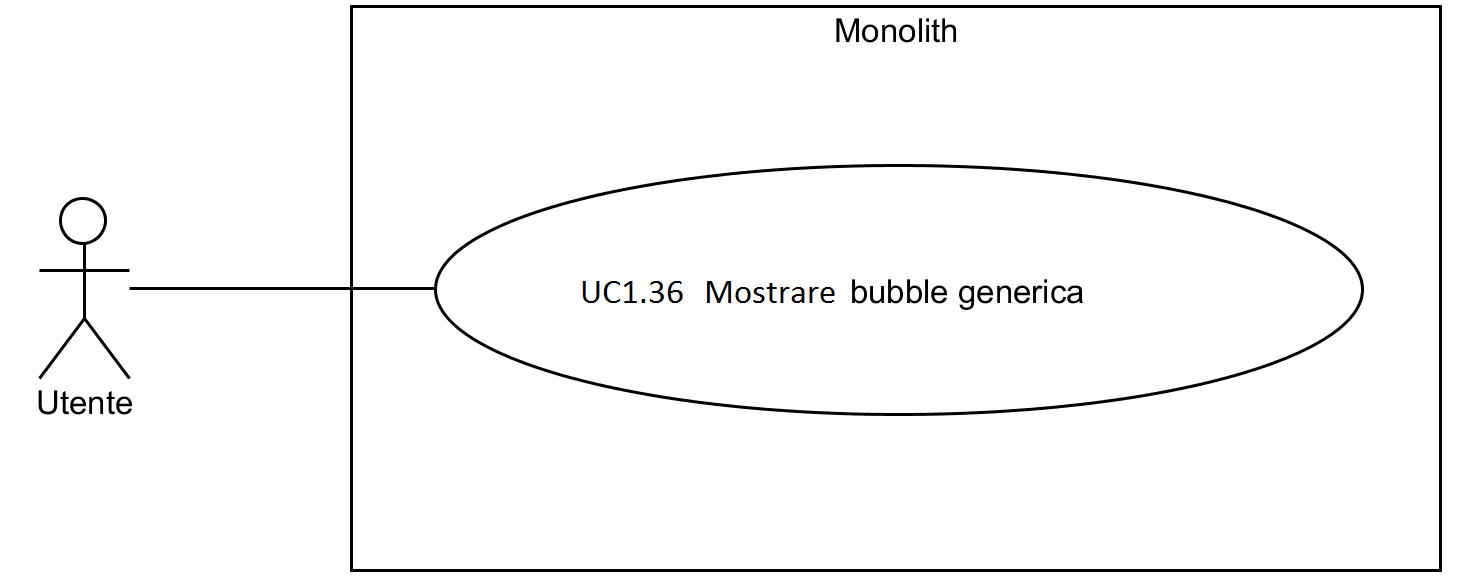
\includegraphics[width=15cm]{../../documenti/AnalisiDeiRequisiti/Diagrammi_img/uc1_36.png}
	\caption{UC1.36 Mostrare bubble generica}
\end{figure}

\begin{itemize}
	\item \textbf{Attori:}
	\begin{itemize}
		\item Utilizzatore del framework;
		\item Rocket.Chat.
	\end{itemize}
	\item \textbf{Scopo e descrizione:} 
	\\L'utilizzatore del framework, utilizzando questo metodo, rende la bubble visibile all'interno della chat.
	\item \textbf{Precondizioni:}
	\begin{itemize}
		\item Avere già istanziato una bubble generica.
	\end{itemize}
	\item \textbf{Flusso principale degli eventi:}
	\\L'utilizzatore del framework chiama il metodo.
	\item \textbf{Post-condizione:}
	\\La bubble specificata viene mostrata all'interno della chat.
\end{itemize}

\UC{Termina bubble}{UC1.19}

\begin{figure}[H]
	\centering
	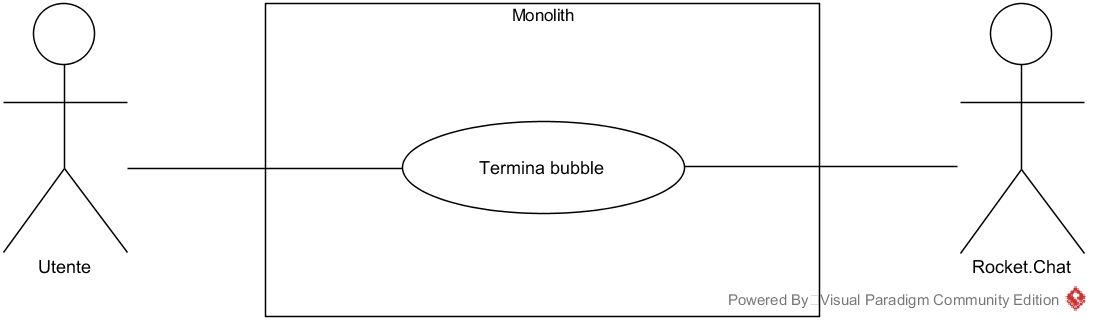
\includegraphics[width=15cm]{../../documenti/AnalisiDeiRequisiti/Diagrammi_img/uc1_19.png}
	\caption{\UCCaption{} Termina bubble}
\end{figure}

\begin{itemize}
	\item \textbf{Attori:}
	\begin{itemize}
		\item Utilizzatore del framework;
		\item Rocket.Chat.
	\end{itemize}
	\item \textbf{Scopo e descrizione:} 
	\\L'utilizzatore del framework potrà terminare la bubble.
	\item \textbf{Precondizioni:}
	\begin{itemize}
		\item Avere già istanziato una bubble generica.
	\end{itemize}
	\item \textbf{Flusso principale degli eventi:}
	\\L'utilizzatore del framework chiama il metodo.
	\item \textbf{Post-condizione:}
	\\La bubble è stata terminata e quindi non sarà più possibile interagire con la stessa. L'interfaccia verrà aggiornata, disabilitando la possibilità di dare input e avere output dinamico ma mantenendo un'istantanea del suo ultimo stato.
\end{itemize}